%% logues.tex
%% Author: Leighton Pritchard
%% Copyright: James Hutton Institute
%% Who let the -logues out?

%
\begin{frame}
  \frametitle{Who let the -logues out?}
  \Large{
    \textcolor{olive}{
      \textbf{
      Genome features can have complex evolutionary relationships \\~\\
      We need precise terms to describe these relationships
      }
    }
  }
  \begin{center}
    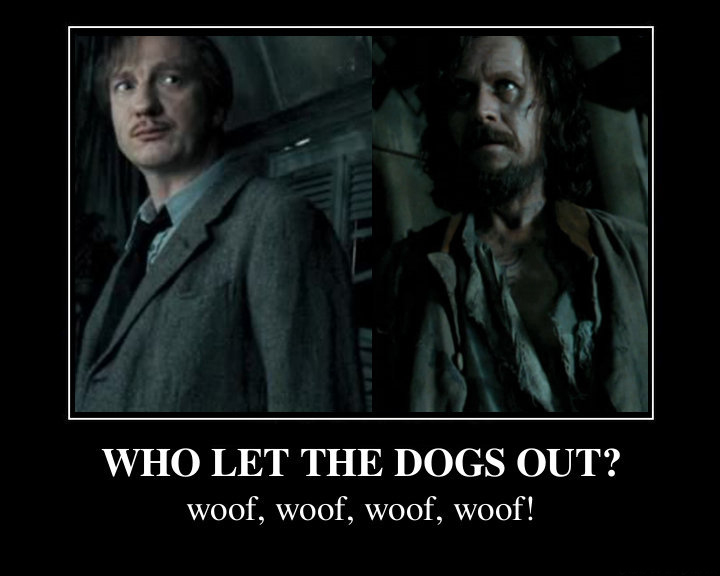
\includegraphics[width=0.4\textwidth]{images/who_let_the_dogs_out}
  \end{center}      
\end{frame}

%
\begin{frame}
  \frametitle{The -logues drop
  \footnote{\tiny{\href{http://dx.doi.org/10.2307/2412448
}{Fitch \textit{et al.} (1970) \textit{Syst. Zool.} doi:10.2307/2412448
}}}
  }
  How do we understand the relationships between features in more than one genome?
  \begin{itemize}
    \item \textcolor{hutton_green}{Functional similarity}: \textbf{analogy}
    \item \textcolor{hutton_blue}{Evolutionary common origin}: \textbf{homology, orthology, etc.}
    \item \textcolor{hutton_purple}{Evolutionary/functional/family relationship}: \textbf{paralogy}
  \end{itemize}
  \begin{center}
    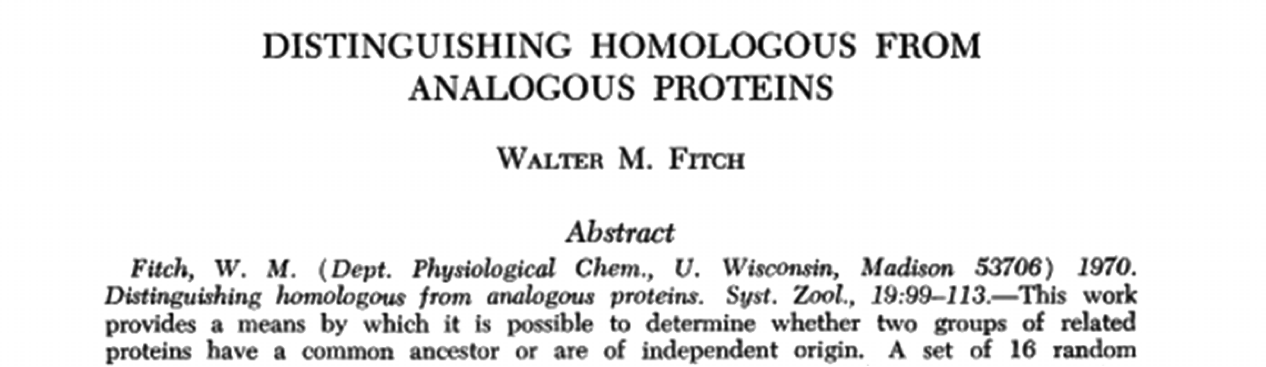
\includegraphics[width=\textwidth]{images/fitch}
  \end{center}    
\end{frame}

%
\begin{frame}
  \frametitle{Definitions
  }
  Technical terms describing evolutionary relationships
  \begin{itemize}
    \item \textbf{\textcolor{hutton_blue}{Homologues}}: share a common ancestor \textcolor{red}{\textbf{NOTE: there are NOT degrees of homology}}
    \item \textbf{\textcolor{hutton_blue}{Analogues}}: are functionally similar. Analogues may or may not share common ancestry
    \item \textbf{\textcolor{hutton_green}{Orthologues}}: are homologues that \textit{diverged through speciation}
    \item \textbf{\textcolor{hutton_purple}{Paralogues}}: are homologues that \textit{diverged through duplication} within the same genome
  \end{itemize}
  (also \textit{co-orthologues}, \textit{xenologues}, etc.)
\end{frame}

% 
\begin{frame}
  \frametitle{Who let the -logues out?}
  \begin{center}
    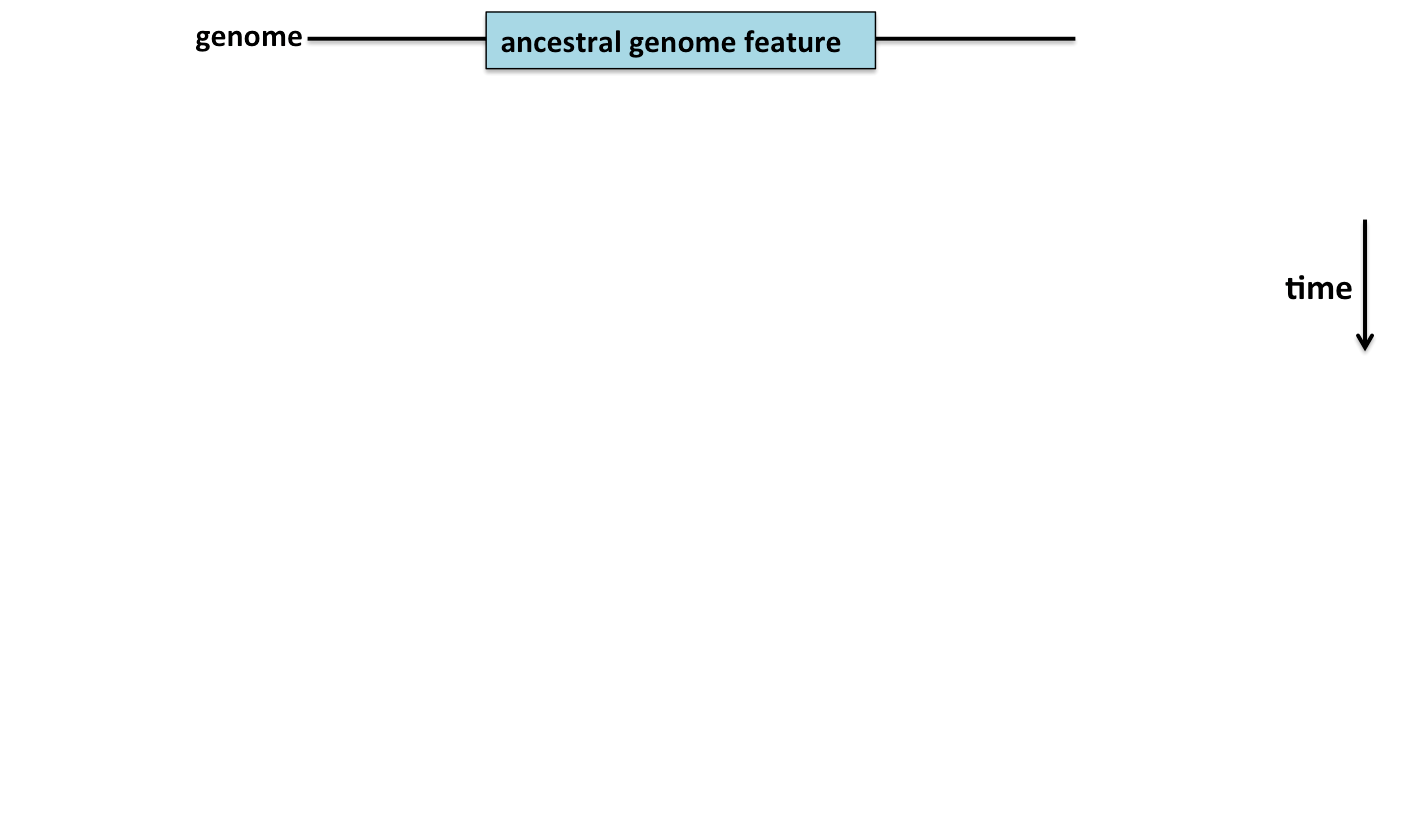
\includegraphics[width=1\textwidth]{images/logues1}  
  \end{center}  
\end{frame}

% 
\begin{frame}
  \frametitle{Who let the -logues out?}
  \begin{center}
    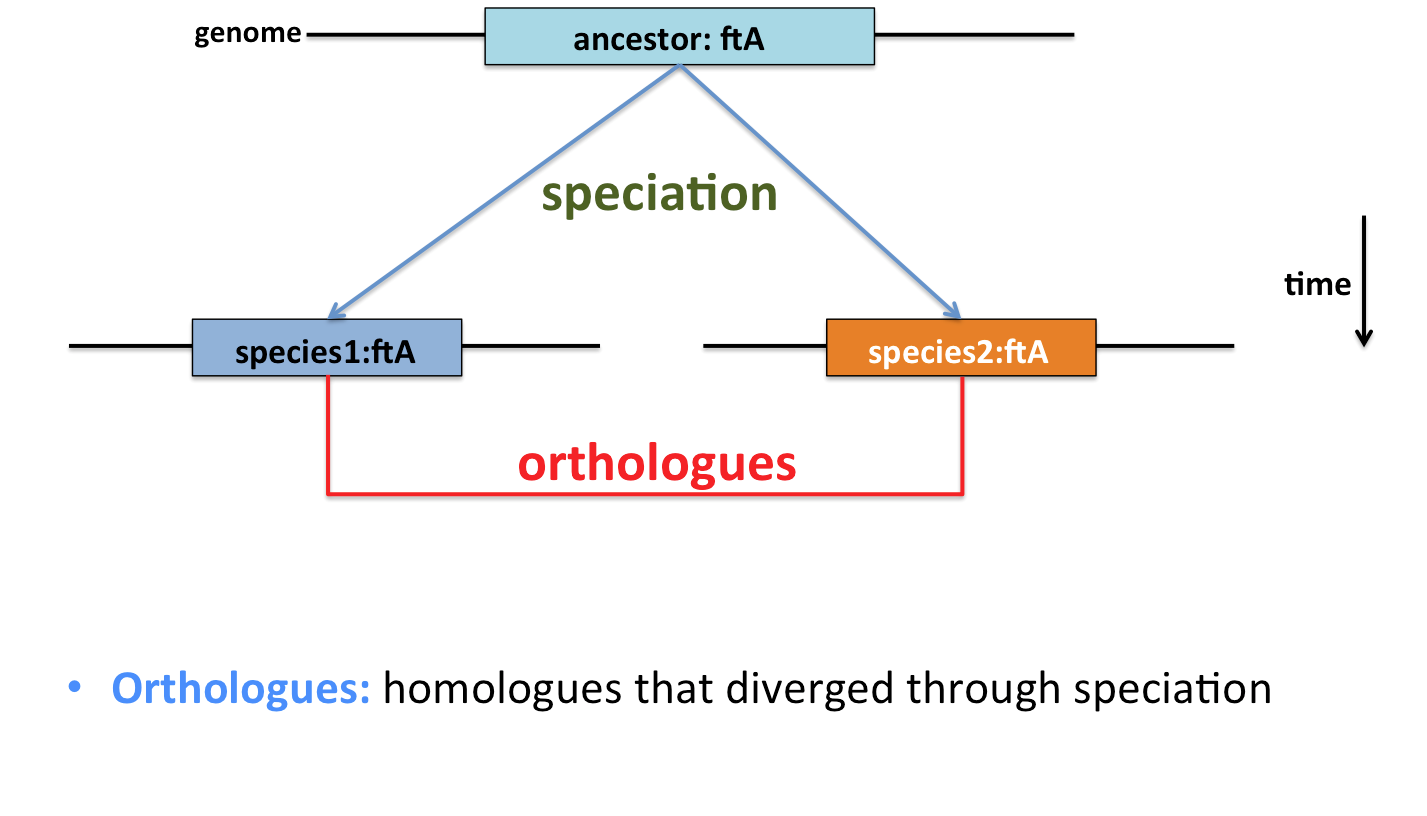
\includegraphics[width=1\textwidth]{images/logues2}  
  \end{center}  
\end{frame}

% 
\begin{frame}
  \frametitle{Who let the -logues out?}
  \begin{center}
    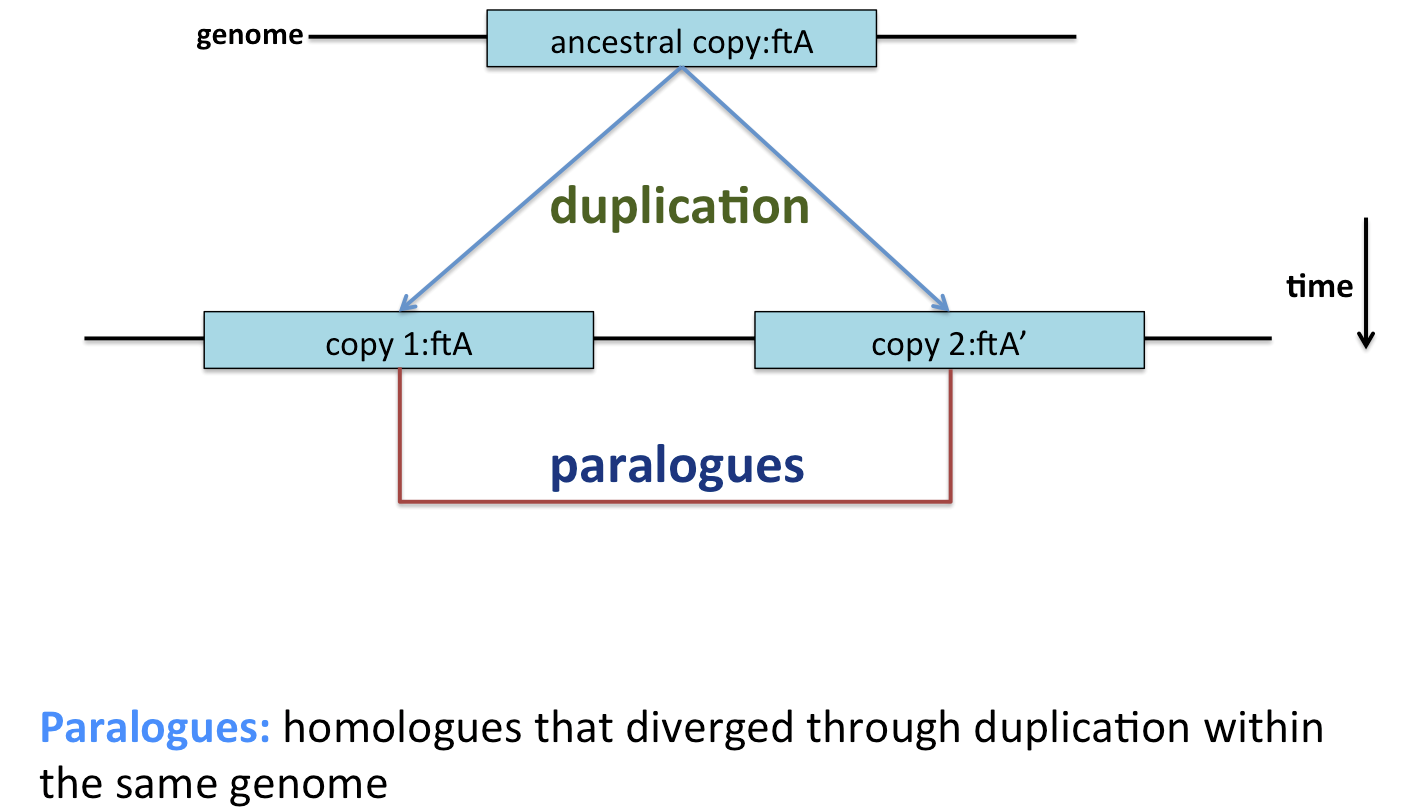
\includegraphics[width=1\textwidth]{images/logues3}  
  \end{center}  
\end{frame}

% 
\begin{frame}
  \frametitle{Who let the -logues out?}
  \begin{center}
    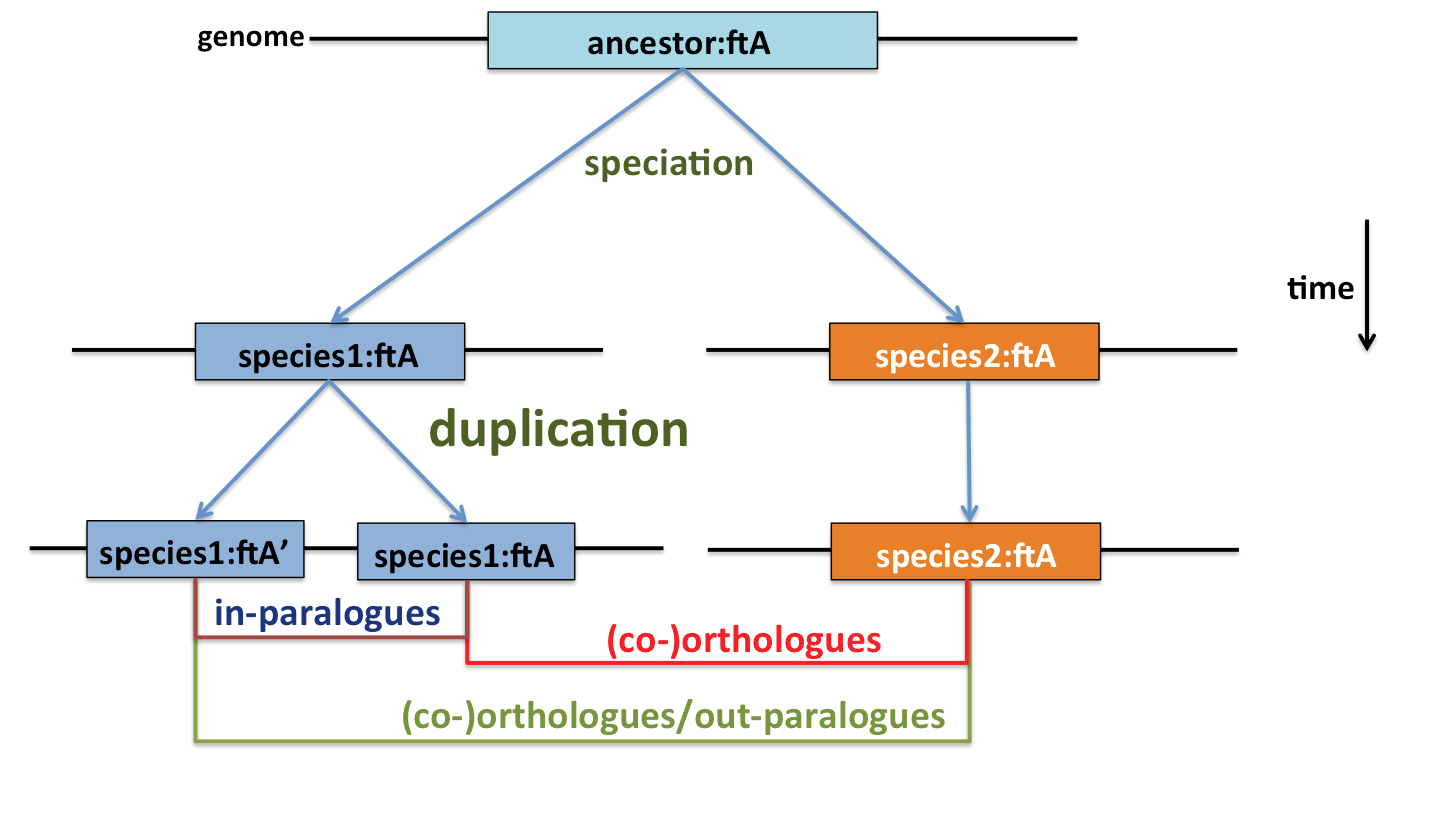
\includegraphics[width=1\textwidth]{images/logues4}  
  \end{center}  
\end{frame}

% 
\begin{frame}
  \frametitle{Who let the -logues out?}
  \begin{center}
    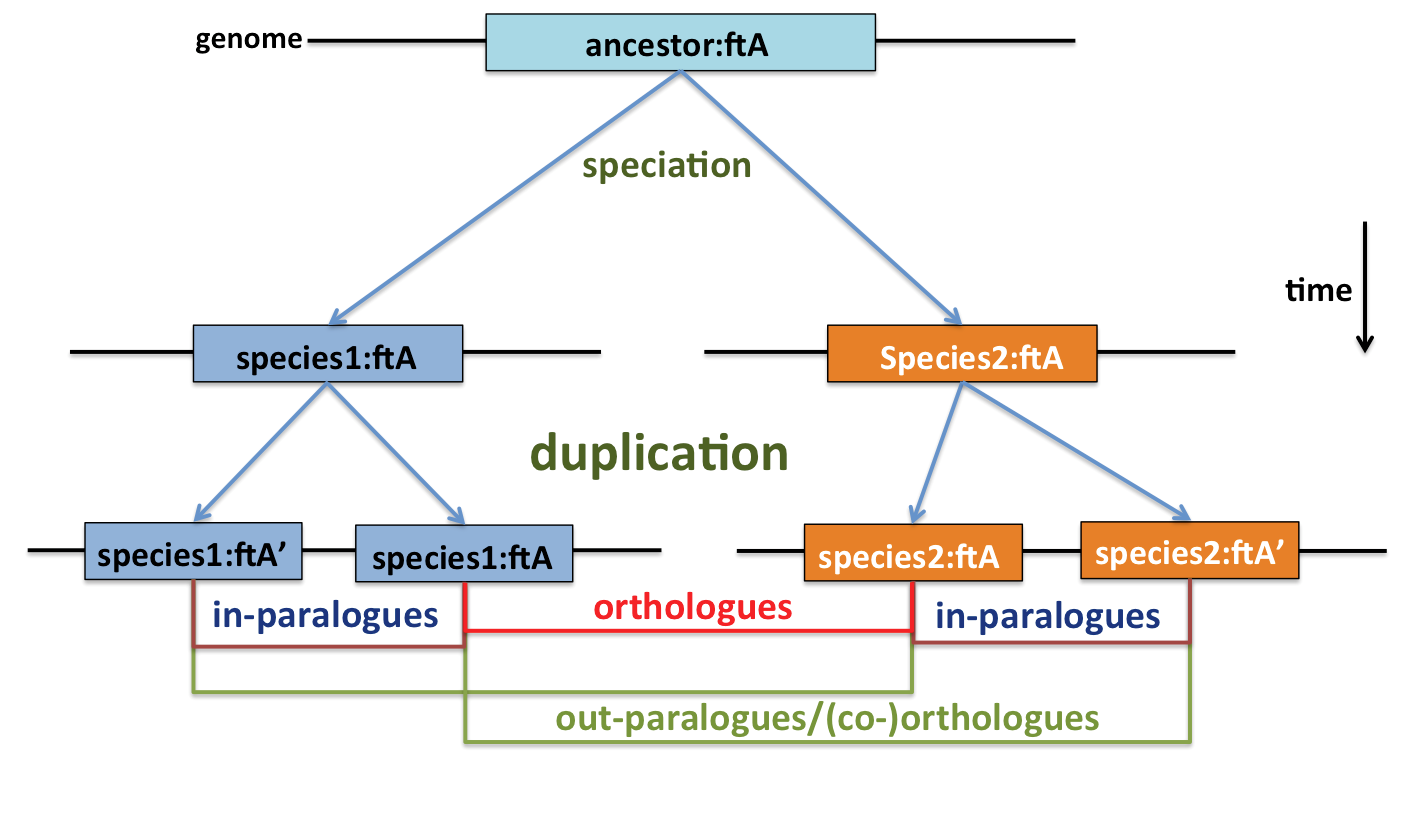
\includegraphics[width=1\textwidth]{images/logues5}  
  \end{center}  
\end{frame}

% 
\begin{frame}
  \frametitle{ITYFIALMCTT\footnote{\tiny{Kristensen \textit{et al}. (2011) \textit{Brief. Bioinf.} \textbf{12}:379-391 \href{http://dx.doi.org/10.1093/bib/bbr030}{doi:10.1093/bib/bbr030}}}}
  But it's a little more complicated than that. \\
  Biology is not well-behaved.
  \begin{itemize}
    \item Gene loss
    \item Homologues may diverge so widely that they can be hard to recognise
    \item Reconstructed evolutionary trees may not be robust inferences of speciation (or relevant to it, in prokaryotes)
    \item There is no record of history - we can only make inferences
  \end{itemize}
  \textbf{All classifications of orthology/paralogy are inferences!}
\end{frame}

% 
\begin{frame}
  \frametitle{ITYFIALMCTT\footnote{\tiny{Kristensen \textit{et al}. (2011) \textit{Brief. Bioinf.} \textbf{12}:379-391 \href{http://dx.doi.org/10.1093/bib/bbr030}{doi:10.1093/bib/bbr030}}}}
  \begin{center}
    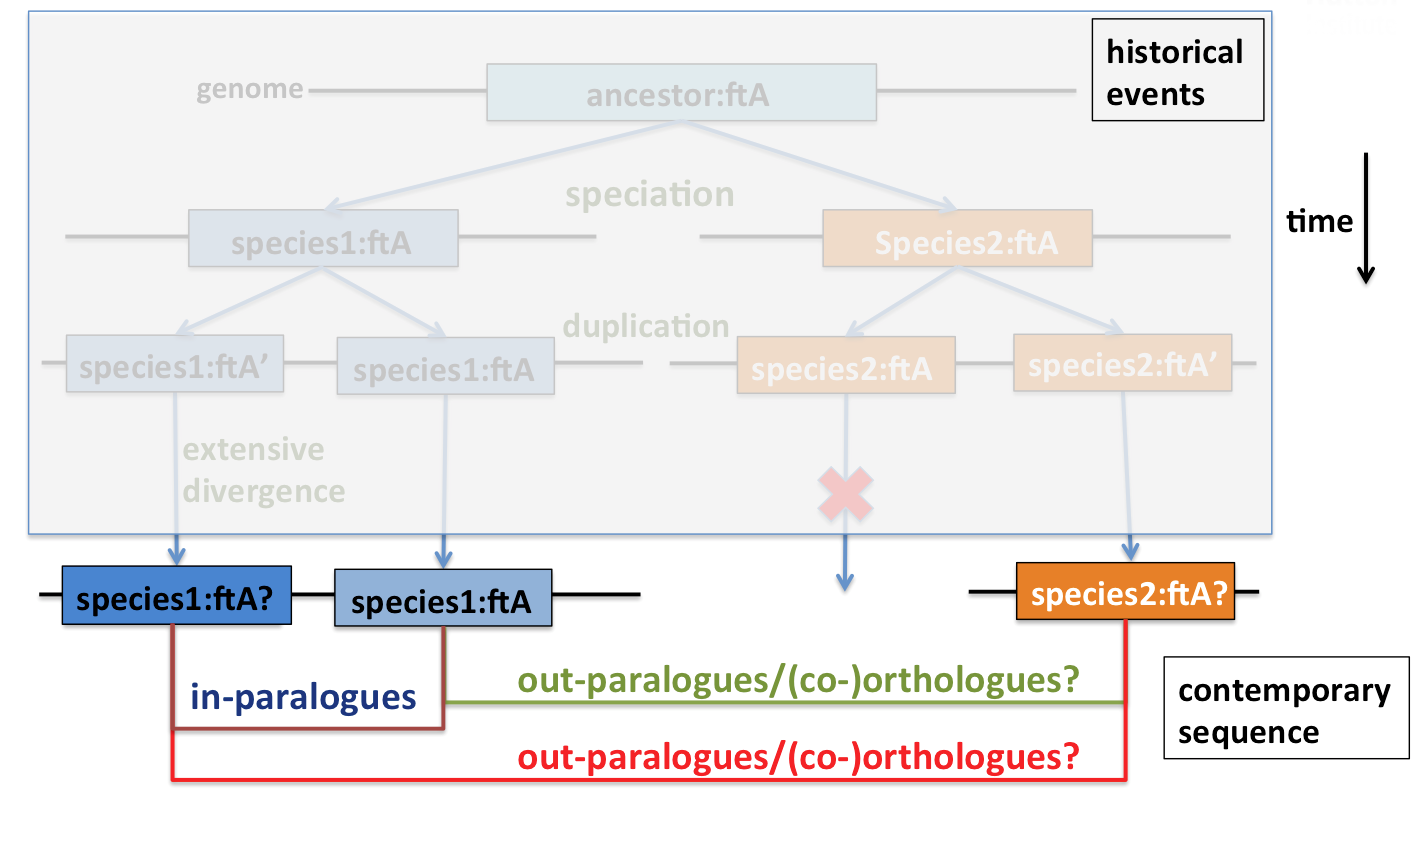
\includegraphics[width=1\textwidth]{images/logues6}  
  \end{center} 
  \textbf{All classifications of orthology/paralogy are inferences!}
\end{frame}

%
\begin{frame}
  \frametitle{Ensembl Compara\footnote{\tiny{Vilella \textit{et al}. (2009) \textit{Genome Res.} \textbf{19}:327-335 \href{http://dx.doi.org/10.1101/gr.073585.107}{doi:10.1101/gr.073585.107}}}}
  Some tools/databases, e.g. \href{http://www.ensembl.org/info/genome/compara/index.html}{Ensembl Compara}, use slightly different definitions (almost everything's an ``orthologue'')
  \begin{center}
    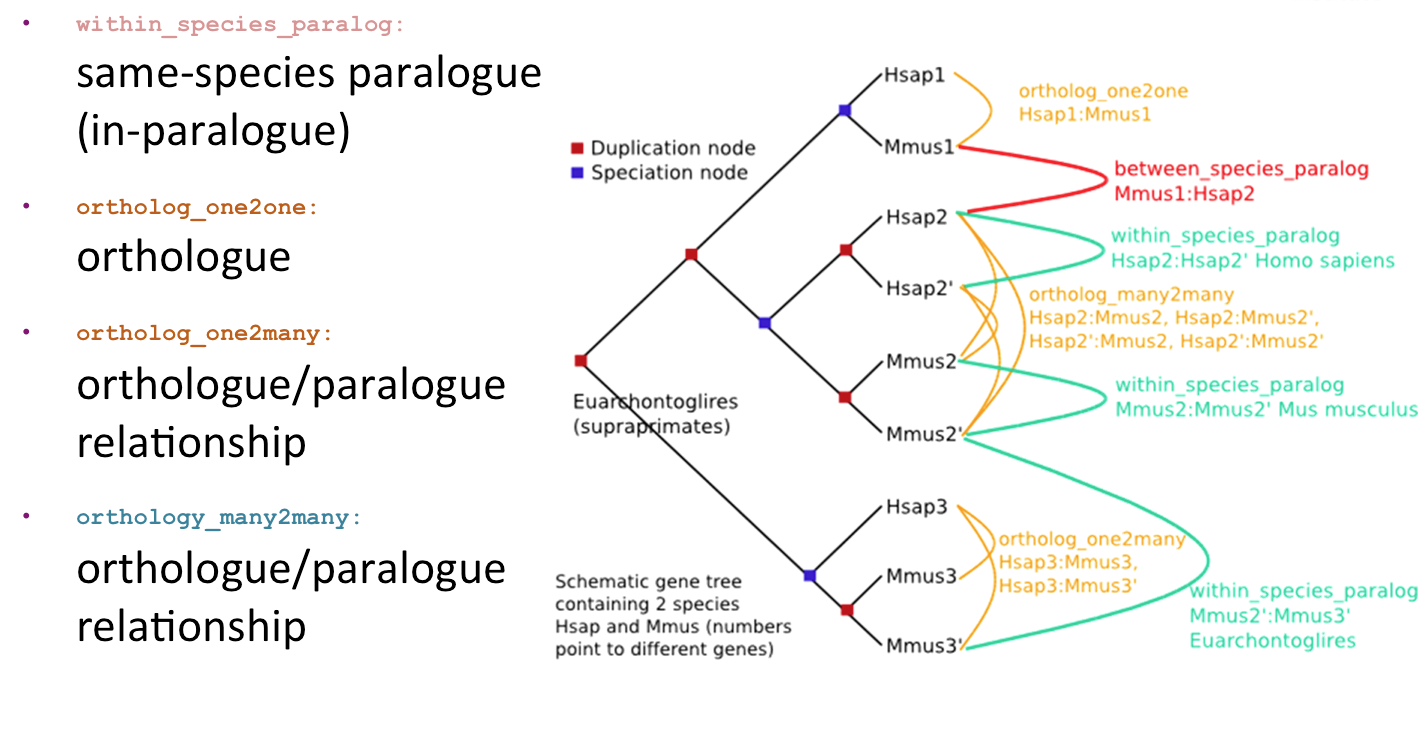
\includegraphics[width=1\textwidth]{images/logues7}  
  \end{center} 
\end{frame}